{
{\sffamily
For at beskrive integrationen og samspillet mellem en kørsel og
databasen vil der følge en beskrivelse af de vigtige kald mellem
programmet og databasen.
}

\subsection{Passende overskrift!!}
Filen \texttt{start.py} er distributør af arbejde til de andre dele af
programkoden.  Diagram \ref{start_workflow} og kodeboks
\ref{pseudo_workflow} giver et overblik over hvad der bliver forklaret i
resten af dette kapitel.

\begin{figure}[h!]
	\begin{center}
		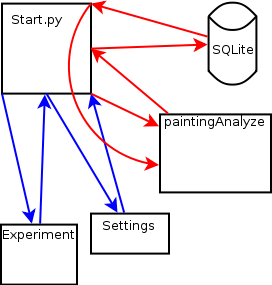
\includegraphics[scale=0.5]{afsnit/implementation/billeder/workflow_start_py.png}
	\end{center}
	\caption{De blå pile er ting, som sker en enkelt gang, mens de blå
	\label{start_workflow}
	bliver gentaget indtil der ikke er flere billeder at arbejde på}
\end{figure}

\begin{lstlisting}[caption={Pseudokode for start}, captionpos=b,
    frame=tb, label={pseudo_workflow}, float=h]
cuts = experiment.generateCuts()
experiment.setSettings(settings)
experiment.setGlobalSettings(globalSettings)
db = Database(globalSettings)
db.construct(Database)
run = m.createNewRun(settings)
paintings = m.Painting.select(m.Painting.q.form=="painting")
for painting in paintings:
    paintingContainer = Painting(painting)
    paintingContainer.setResults(
            paintingAnalyzer.analyze(paintingContainer,settings))
    m.saveResults(run.id,paintingContainer)
\end{lstlisting}
\subsection{Eksperimenter}
Eksperimenter angiver hvilke snit og indstillinger en given kørsel skal
afvikles med. I kodeboks \ref{pseudo_experiment} ses et eksempel på,
hvordan et eksperiment kan se ud.

\begin{lstlisting}[caption={Pseudokode for et experiment, som checker på
    $\varPhi$ og $\frac{2}{3}$}, frame=tb, label={pseudo_experiment},
    captionpos=b, float=h]
def generateCuts():
	cuts = [goldenLibrary.PHI, 2.0/3.0]
	return cuts

def setSettings(settings):
	settings.setMarginPercentage(0.024)
	return 0

def setGlobalSettings(globalSettings):
	return 0
\end{lstlisting}

\subsection{Globale indstillinger}
I de globale indstillinger sættes placeringen på databasen og den
kommaseparerede fil. Dette er indstillinger, som ikke påvirker en kørsel
direkte, altså en ændring i disse værdier ville producere præcis
den samme kørsel, som før ændringerne. 

\subsection{Kørselsindstillinger}
Kørselsindstilinger kan ændre sig i de forskellige kørsler. De består af
tærskelværdier for floodfill og kantdetektion, hvilken analysemetode vi
ønsker at bruge, samt størrelsen på margin og de snit, som skal
undersøges. De her variabler betyder meget for resultaterne og derfor er
vigtige at kunne ændre fra kørsel til kørsel.

\subsection{Initialisering af databasen}
Databasen er kopieret fra et online kunstarkiv kaldet ``The Web Gallery
of Art''\cite{wgahu}, forkortet WGA. WGA supplerer en kommasepareret fil, med
maleriernes metadata, som vi bruger til at populere vores database med.
Ved at bruge \emph{SQLObject} er det ligetil at konstruere tabeller i
databasen. Vi har i afsnit \ref{section_database} givet det database
skema som vi opbygger databasen efter. I kodeboks
\ref{code_tabel_artist} er vist hvordan tabellen \texttt{artist}
konstrueres ved brug af \emph{SQLObject} i Python.

\begin{lstlisting}[caption={Pythonkode for oprettelse af tabeller i
    databasen.}, captionpos=b, label={code_tabel_artist}, frame=tb,
    breaklines=false, float=hb]
import sqlobject as s

class Artist(s.SQLObject):
    "
    _id_, name, born, died, school, timeline
    "
    name = s.StringCol()
    born = s.IntCol()
    died = s.IntCol()
    school = s.StringCol()
    timeline = s.StringCol()
\end{lstlisting}

Når man vil oprette en ny kunstner i databasen gøres det som vist
i kodeboks \ref{code_new_artist}.

\begin{lstlisting}[caption={Oprettelse af en kunstner i databasen.},
    captionpos=b, label={code_new_artist}, frame=tb, breaklines=false,
    float=h]
# Init variables
name = "Homer Simpson"
born = 1968
died = 2000
school = "Springfield"
timeline = "1950-2000"

# Create the artist in the database
Artist(name=name, born=born, died=died, school=school, timeline=timeline)
\end{lstlisting}

\emph{SQLObject} opretter automatisk et id-felt til alle tabeller i
databasen. Vi kan udnytte dette til at lave \emph{foreign keys} i
tabellerne. Vi viser i kodeboks \ref{code_tabel_result} hvordan tabellen
\texttt{result} oprettes i databasen, hvor det er interessant at bemærke
hvorledes de to \emph{foreign keys} oprettes.

\begin{lstlisting}[caption={Pythonkode for oprettelse af \emph{foreign
    keys} i databasen.}, captionpos=b, label={code_tabel_result}, frame=tb,
    breaklines=false, float=h]
class Result(s.SQLObject):
    "
    _id_, ^runId, ^paintingId, cutRatio, cutNo, numberOfRegions
    "

    run = s.ForeignKey('Run')
    painting = s.ForeignKey('Painting')
    cutRatio = s.FloatCol()
    cutNo = s.IntCol()
    numberOfRegions = s.IntCol()
\end{lstlisting}

Den kommaseparerede fil bliver parset før enhver kørsel, og bliver, linje for linje, sammenlignet med
databasen for at finde evt. mangler. Hvis det er første gang en kørsel
sættes igang, ville databasen derfor blive bygget op.  Bemærk, at databasen ikke kan
håndtere at blive afbrudt i dette stadie, første gang den bliver kørt,
fordi det er en meget overfladisk sammenligning, hvor kun billeders
placering på \url{http://www.wga.hu}, som bliver sammenlignet, da denne
er unik.  Omvendt giver det mulighed for at den kommaseparerede fil kan
opdateres uden nogen problemer. Nye billeder bliver automatisk hentet,
hvilket gør det muligt, at flytte databasen til en anden maskine, uden
problemer. Der er kun to tilfælde hvor databasen kan håndtere
udvidelser; hvis den kommasepareredefil bliver opdateret og beholder sin
nuværende form, og hvis en testdatabases \texttt{count}-variabel bliver
sat til en højere værdi. Det sidste tilfælde forklares senere.  Følgende
pseudokode, i kodeboks \ref{pseudo_init_db}, forklarer hvad databasen
gennemgår, hver gang der startes en ny kørsel.

\begin{lstlisting}[caption={Pseudokode for database
    initialisering},frame=tb,label={pseudo_init_db}, captionpos=b,
    float=h]
csvfile = open(Settings.csvfilelocation)
for line in csvfile:
	line = parser.parse(line)
	if not os.path.isfile(line.path):
		download(line.url)
	if database.Painting.select(database.Painting.url==line.url).count() == 0:
		database.Painting.insert(line)
\end{lstlisting}

\subsubsection{Parsing af kommasepareret fil}
I den kommaseparerede fil gives mange oplysninger, om den enkelte
artikel samt dennes kunstner.  Vi har konstrueret en parser, som trækker
disse informationer ud fra filen og lægger dem ind i databasen. Da vi
primært vil beskæftige os med malerier, vil vi nu blot omtale
kunstartikler som malerier.

Den konstruerede parser, til den kommaseparerede fil, er dog ret grov,
da folkene bag WGA ikke har lagt meget vægt på, at være konsistente i
deres formulering af en kunstners fødsels- og dødsår eller en genstands
dimensioner. En følge deraf er, at nogle kunstnere, hvor WGA ikke har en
klar indikation af dennes levealder, ikke bliver registreret i
databasen. Vi kan dog stadig slå kunstneren op ved at bruge feltet
``timeline'', som angiver hvilken periode kunstneren tilhører. Vi har i
enkelte tilfælde, set os nødsaget til at rette i den kommaseparerede
fil, når der er blevet indsat tegn, som helt umuliggør korrekt parsing
af filen, såsom ekstra komma eller semikolon.

\subsubsection{Testdatabase}\label{test_db}
For at alle kan arbejde på de samme billeder undervejs i udviklingen, er
det muligt at konstruere en lille testdatabase, måden det gøres på i
denne implementering kan ses i brugervejledningen
\ref{brugervejl_test_db}. Da flere personer skal
kunne sammenligne deres evt. resultater bør den samme testdatabase
bliver skabt hvis parametrene sættes til det samme.

\subsection{Analysen}
Analysen bliver kørt på alle billeder, som har typen ``painting'' i den
kommaseparerede fil. Som beskrevet i linje 8--10 i kodeboks
\ref{pseudo_workflow}, bliver billedet sendt igennem klassen
\textbf{Painting}, hvor det bliver konverteret til et
\emph{OpenCV}-billede. Når det er konverteret sendes det til
\texttt{paintingAnalyzer}, hvis formål er at sende det videre til
udtrækning af regioner, alt efter hvilken analysemetode der bruges,vist
med pseudokode i \ref{pseudo_naiveMethod}. Alle snittene løbes igennem
for regioner.
Når alle regioner er trukket ud, gemmes resultaterne i databasen.

\begin{lstlisting}[caption={Pseudokode til analyse af malerier efter
    metode}, captionpos=b, label={pseudo_naiveMethod}, frame=tb,
    breaklines=false, float=h]
def AnalyzePainting(painting, settings):
    # Get the method used for the analysis
    method = settings.method

    # Use the right method
    if method == 'naive':
        image = painting.getImage()
        return NaiveMethod(image, settings)
    else if method == 'expanded':
		image = painting.getImage()
		return ExpandedMethod(image,settings)
	else:
        print 'No such method'
        return None
\end{lstlisting}

\begin{lstlisting}[caption={Pseudokode for den naive metode},
    captionpos=b, label={pseudo_naiveMethod}, frame=tb,
    breaklines=false, float=h]
def NaiveMethod(image, settings):
    # Init ImageRegions dict
    ImageRegions = {}

    # Walk through all the CutRatios
    for CutRatio in settings:
        # Init RatioRegions dict
        RatioRegions = {}

        # Walk through every Cut in the ratio
        for Cut in CutRatio:
            # Set up the constraints, extract regions and prune the regions
            Constraints = new Constraints(image, Cut, settings)
            CutRegions = NaiveExtraction(image)
            InterestingRegions = GetInterestingRegions(CutRegions, Constraints)
            InterestingRegionsInCut =
                    GetInterestingRegionsInCut(InterestingRegionsInCut, Constraints)

            # Put the resulting instance of CutRegions
            # in the Regions-dict
            RatioRegions[Cut] = InterestingRegionsInCut

        # Put the resulting RatioRegions in the ImageRegions-dict
        ImageRegions[CutRatio] = RatioRegions

    # Return the resulting ImageRegions-dict
    return ImageRegions
\end{lstlisting}

\subsection{Genskabelse af parametre og resultater}
\note{Jeg tror ikke at det følgende er blevet læst igennem til at passe
til dette afsnit.}
At kunne genskabe de fundne resultater fra en analyse har meget stor
betydning, dels for at kunne udtage stikprøver i udviklingen af hele
programmet, men også for at kunne fremvise grafiske resultater. Vi har
allerede været inde på, at man, for at kunne genskabe et resultat, skal
vide hvilke parametre der oprindeligt har været brugt.Hvis vi får et
resultat med overraskende mange regioner og gerne vil undersøge dette
tilfælde, har vi metoder til rådighed der giver os lige nøjagtig de
informationer vi har brug for at vise dette grafisk. Helt konkret har vi
metoderne vist i listing \ref{rekonst_koersel} til rådighed.

\vspace{0.5cm}
\begin{lstlisting}[caption={Metoder til rekonstruktion af kørsler},captionpos=b,label={rekonst_koersel},numbers=none]
def getSettingsForRunId(runId):
    """Return the settings instance for a given run"""
    pass

def getCutRatiosForRunId(runId):
    """Return the list of cut ratios for a given run"""
    pass

def getSettingsForResultId(resultId):
    """Return the settings instance for a given result"""
    pass

def getSettingsForRegionId(regionId):
    """Return the settings instance for a given region"""
    pass

def getCutRatioForRegionId(regionId):
    """Return the list of cut ratios for a given region"""
    pass

def getCutNoForRegionId(regionId):
    """Return the cut number for a given region"""
    pass

def getRegionsForResultId(resultId):
    """Return the list of regions for a given result"""
    pass
\end{lstlisting}

Selvom metoderne i listing \ref{rekonst_koersel} ikke viser noget
egentlig kode, bør det ud fra sammenhængen være klart hvad disse metoder
gør. Alle metoder der starter med \texttt{getSettings} returnerer
klassen \texttt{Settings} som vist i listing \ref{settings_klassen} med
indstillinger tilpasset den enkelte forespørgelse.
\vspace{0.5cm}
\begin{lstlisting}[caption={Settings-klassen med standardindstillinger},captionpos=b,label={settings_klassen},numbers=none]
class Settings:
    """These are the default settings for the analysis"""
    edgeThreshold1 = 78
    edgeThreshold2 = 2.5 * edgeThreshold1
    lo = 4
    up = 4
    cutRatios = None
    marginPercentage = 0.009
    method = 'naive'
    ...
\end{lstlisting}

Det ses at vi har mulighed for at trække de fundne regioner ved et
snit ud og vi behøver derfor ikke at køre nogen analyse på billedet hvis
vi blot ønsker at få de fundne regioners begrænsende areal vist. I dette
tilfælde kan vi nøjes med at forespørge databasen om de regioner der er
tilknyttet et snit vi gerne vil undersøge og traversere gennem den liste
af regioner vi får tilbage. Hver region er repræsenteret som en klasse
hvor vi kan trække rektanglet ud og vi bruger da \emph{OpenCV} til at
tegne rektanglet på det tilknyttede billede.
}
% vim: set tw=72 spell spelllang=da:
